\chapter{\label{method}Theory}
In this chapter, the theoretical background will be detailed before we discuss the particulars of the experiment.
\section{Magnetostriction}
The internal structure of ferromagnetic materials is composed of domains, each of which is a region of uniform magnetization. The domain boundaries move and the domains rotate when a magnetic field is applied; both of these effects change the material's dimensions. Because it requires more energy to magnetize a crystalline material in one direction than in another, magnetocrystalline anisotropy\footnote{A ferromagnetic material is said to have magnetocrystalline anisotropy if it takes more energy to magnetize it in certain directions than in others.} is the reason that altering a material's magnetic domains causes a change in the material's dimensions. The material will tend to rearrange its structure so that an easy axis is aligned with the field to minimize the free energy of the system if a magnetic field is applied to it at an angle to an easy axis of magnetization\footnote{Easy axis refers to the energetically favorable direction of the spontaneous magnetization in a ferromagnetic material.}. This differential induction of direction leads to strain in the material.

In fact, the reciprocal effect is also observed in the form of Villari effect, which is defined as the change in the magnetic susceptibility (which quantifies the response to an applied field) of a magnetic material under some form of mechanical stress. The Matteucci and Wiedemann effects are also two related phenomena where mechanical transformation of ferromagnetic materials leads to changes in their magentic properties.

The changes in dimensions of the material are always in the direction of magnetization, and it they can be positive or negative depending on if the material is contracting or elongating. The distortions are usually of the order $10^{-8}$ to $10^{-4} \si{\meter}$, is due to spin-orbit mutual potential energy and is a function of the direction of magnetisation and the interatomic distances.
\section{LASER}
A laser is a device that emits a narrow beam of coherent light with small angular dispersion. It works on the principle of stimulated emission. The basic concept is to have the electrons in an inverted state where most of them are in the excited levels in a gain medium (crystal or gas). Light is created when this medium is excited by an external energy source (stimulation). This leads to chain reaction where the population inversion reverses and all the electrons fall to the ground level. The photons travel back and forth through a resonant cavity, which contains mirrors at both ends, and are amplified with each pass through the gain medium.\\
In our experiment, we are using the He-Ne laser. The stimulation is a small electric current and the final colour of the beam produced is red (\SI{632.8}{\nano \meter}).
\begin{figure}[H]
	\centering
	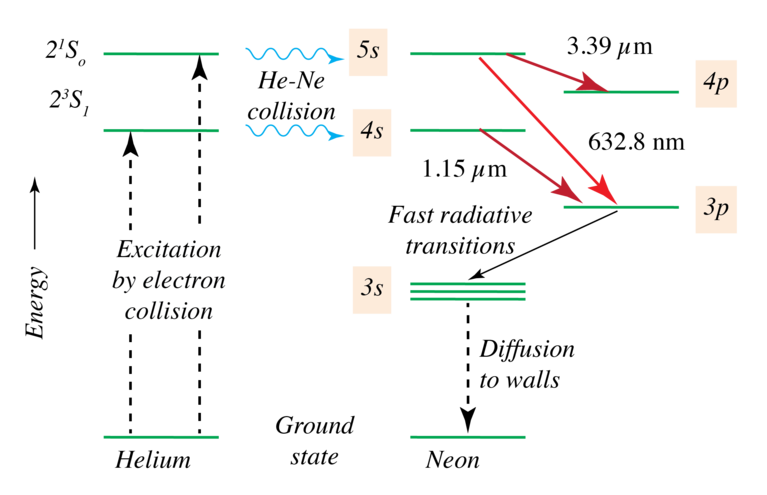
\includegraphics[width=0.7\textwidth]{hene.png}
	\caption{Energy Levels in the lasing medium}
	\label{fig:flow around cylinder}
	
\end{figure}
\begin{figure}[H]
	\centering
	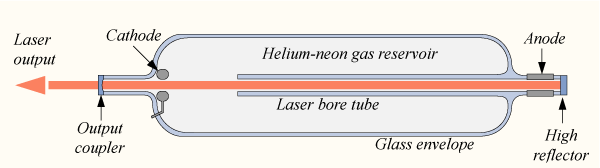
\includegraphics[width=0.7\textwidth]{hene1.png}
	\caption{Construction of the laser}
	\label{fig:flow around cylinder}
	
\end{figure}
\section{Michelson Interferometer}
The Michelson interferometer is one of the most important devices that is used to measure small distances.

The basic setup of a Michelson interferometer consists of a beam splitter, two mirrors, and a detector. A beam of light is split by the beam splitter, with half of the light directed towards one mirror and half towards the other mirror. The mirrors reflect the light back towards the beam splitter, where the two beams are recombined. The interference between the two beams produces an interference pattern that can be observed at the detector.

By varying the distance between one of the mirrors and the beam splitter, the interference pattern can be changed. This allows the Michelson interferometer to be used for a variety of measurements. By measuring the change in interference pattern as the sample is moved, the length change can be obtained.
To obtain the equation for the interference pattern, we use the concept of superposition of waves.
\begin{equation}
	2 d \cos \theta = m \lambda
\end{equation}
This means that for a given theta, the number of fringes that cross a point depends on how d changes. Hence, we can count the number of fringes changed to find out the change in distance of the mirror.
\begin{figure}
	\centering
	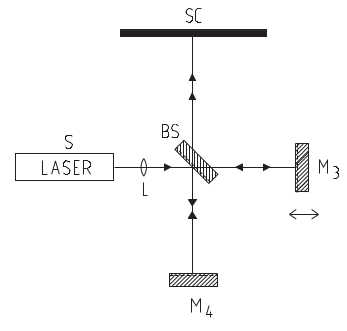
\includegraphics[width=0.7\linewidth]{mich}
	\caption{Michelson arrangement for Interference. \textbf{S} represents
		the light source; \textbf{SC} the detector (or the position of the
		screen)}
	\label{fig:mich}
\end{figure}

Magnetostriction can be described thermodynamically using $S$ (elastic tension), $s$ (deformation $\Delta l/l$), $B$ (magnetic induction), $H$ (magnetic field strength), $\mu$ (magnetic permeability) as
\begin{center}
	$\dfrac{1}{\mu} = \dfrac{\partial H}{\partial B}$,
\end{center}
$E$ (elasticity module) with
\begin{center}
	$E = \dfrac{\partial S}{\partial s}$,
\end{center}
as
\begin{equation}
	\dfrac{\partial S}{\partial s} = \dfrac{1}{4 \pi} \cdot \dfrac{\partial H}{\partial s}
\end{equation}
\section{Photo-diode Detector}
A photodiode detector is a type of semiconductor device that is used to detect light or optical signals. Photodiode detectors are made from a special type of semiconductor material, such as silicon or germanium, which is doped to create a p-n junction. When light enters the photodiode, it creates electron-hole pairs in the depletion region of the p-n junction. The resulting current that flows through the photodiode is proportional to the amount of light that is detected.
\begin{figure}[H]
	\centering
	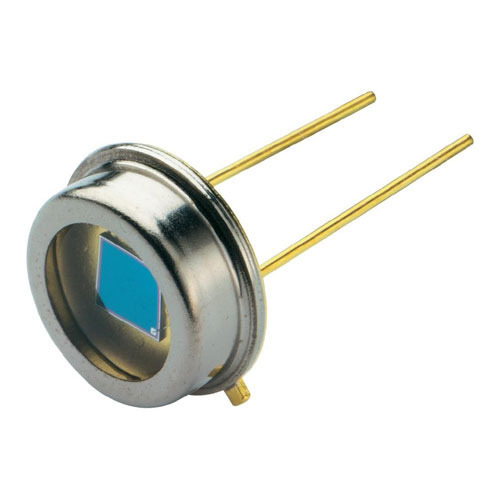
\includegraphics[width=0.4\textwidth]{photo.jpg}
	\caption{Photodiode Detector}
	\label{fig:flow around cylinder}
\end{figure}
If there is a bright fringe incident on the detector, there will be an output voltage signal which can be recorded. In the case of a dark fringe, we will not observe any voltage output. 
\begin{figure}[H]
	\centering
	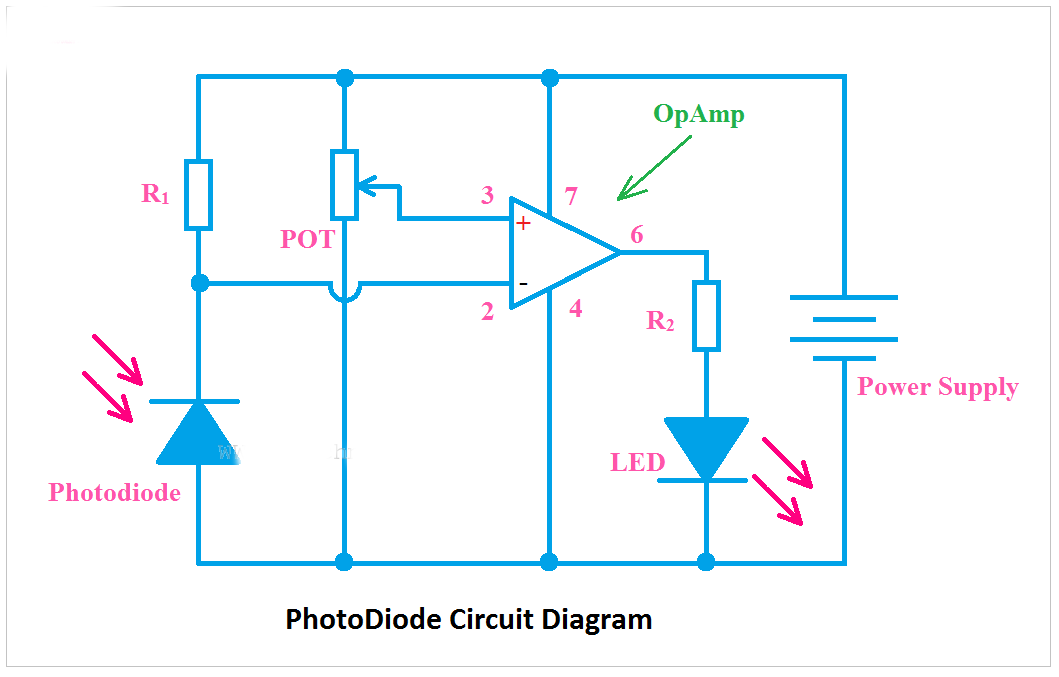
\includegraphics[width=0.7\textwidth]{photcircuit.png}
	\caption{Photodiode Detector Circuit with Amplifier}
	\label{fig:flow around cylinder}
\end{figure}
In our particular case, we use an op-amp. Whenever the photodiode senses light, it generates a voltage. In this setup, an op-amp serves as a comparator. It compares the voltage generated by the photodiode to the reference voltage supplied by the Vcc or main power supply and produces output accordingly.
\setcounter{equation}{0}
\setcounter{table}{0}
\setcounter{figure}{0}
%\baselineskip 24pt


    



